\chapter{Конструкторская часть}

В данном разделе будут указаны требования к программному обеспечению и представлены схемы алгоритмов нахождения расстояния Левенштейна и Дамерау-Левенштейна.

\section{Требования к ПО}

К программе представлен ряд требований:

\begin{itemize}
	\item на вход подается массив целых чисел в диапазоне [-1000;1000];
	\item на выходе - отсортированный массив, поданный на вход. При сортировке изменяется изначальный массив, а не его копия.
\end{itemize}

\section{Разработка алгоритмов}

На рисунках \ref{img:selection_sort}, \ref{img:shell_sort}, \ref{img:gnome_sort} представлены схемы алгоритмов сортировки выбором, Шелла и гномьей сортировки.

\begin{figure}[H]
	\begin{center}
		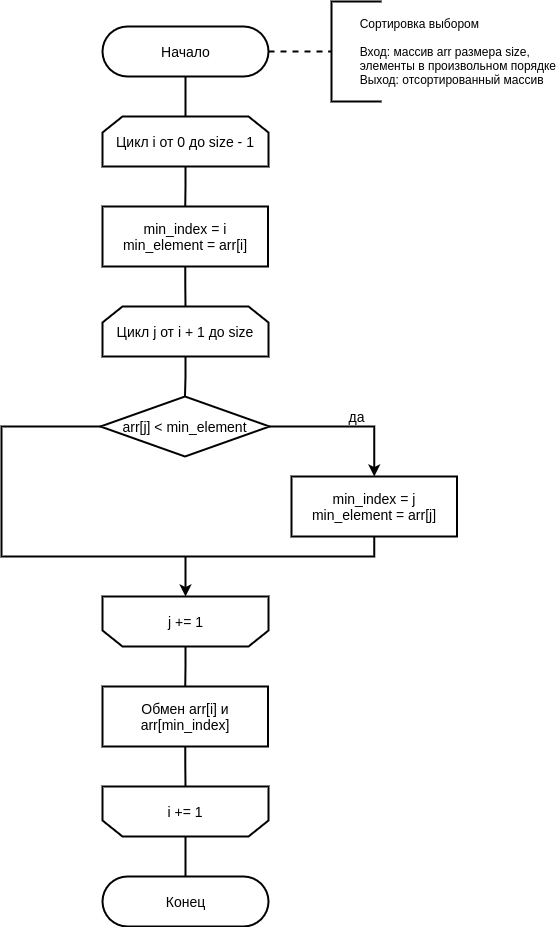
\includegraphics[scale=0.4]{img/selection_sort.png}
	\end{center}
	\captionsetup{justification=centering}
	\caption{Схема алгоритма сортировки выбором}
	\label{img:selection_sort}
\end{figure}

\begin{figure}[H]
	\begin{center}
		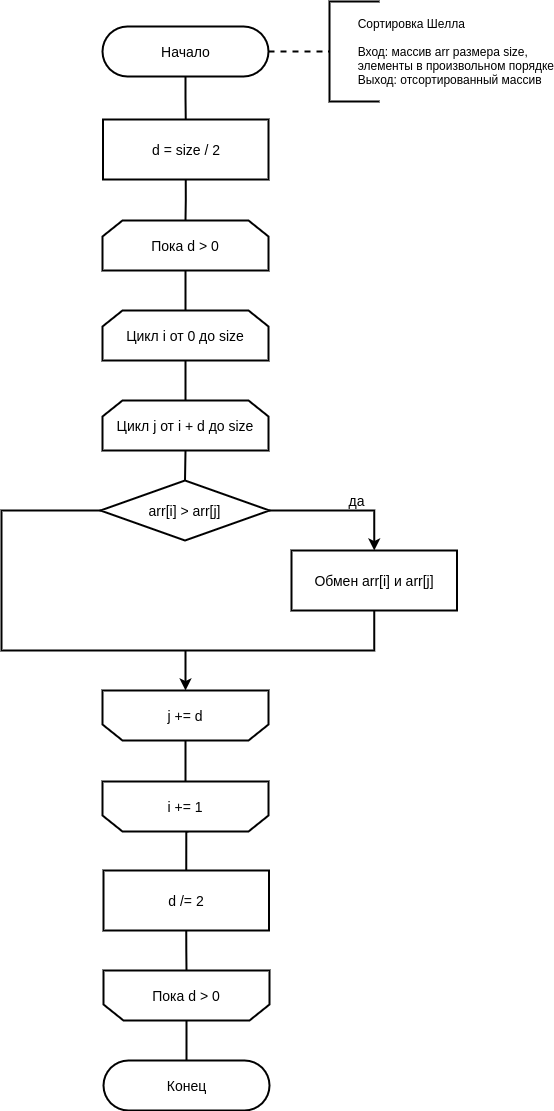
\includegraphics[scale=0.5]{img/shell_sort.png}
	\end{center}
	\captionsetup{justification=centering}
	\caption{Схема алгоритма сортировки Шелла}
	\label{img:shell_sort}
\end{figure}

\newpage

\begin{figure}[H]
	\begin{center}
		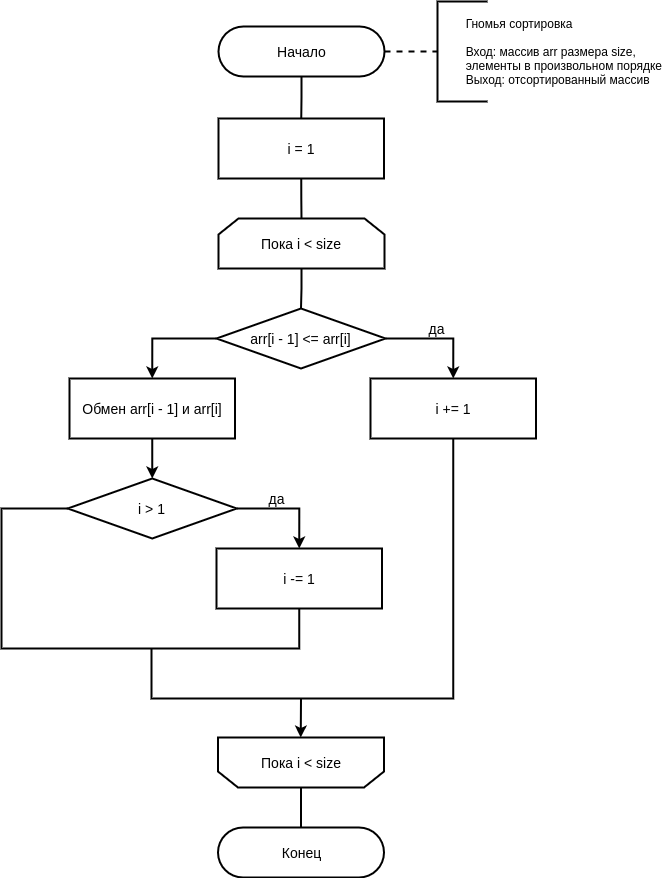
\includegraphics[scale=0.5]{img/gnome_sort.png}
	\end{center}
	\captionsetup{justification=centering}
	\caption{Схема алгоритма гномьей сортировки}
	\label{img:gnome_sort}
\end{figure}

\section*{Вывод}

Были представлены схемы алгоритмов сортировки выбором, Шелла и гномьей сортировки и указаны требования к ПО.
